\documentclass{article}
\usepackage{graphicx} % for including graphics
\usepackage[utf8]{inputenc}
\usepackage{geometry} % For page size and margins
\geometry{a4paper, margin=0.8in}

\title{Database Design Report for Hotel Management System | Assignment 02}
\author{Muhammad Rehan | 22P-9106}
\date{2 May 2024}

\begin{document}

\maketitle

\begin{abstract}
This report details the database design process for a hotel management system, highlighting the development of ER diagrams and SQL schema. The objective is to make hotel operations and guest experiences good through an effective database system.
\end{abstract}

\section*{Introduction}
Advanced database systems have changed hotel management. The work in this assignment develops a comprehensive database to support room booking, inventory control, and staff management.

\section*{System Overview}
The designed system manages operations across multiple hotel properties, enhancing efficiency in room bookings, staff deployment, and inventory control.

\section*{ER Diagrams}
\subsection*{Conceptual Model}
The conceptual ER diagram provides an overview of the entities and their basic relationships. The diagram is at the end of the doc.


\subsection*{Logical Model}
The logical ER diagram details the relationships and attributes. The diagram is at the end of the doc.


\subsection*{Physical Model}
The physical ER diagram is tailored for MySQL implementation, specifying data types and constraints. The diagram is at the end of the doc.


\section*{Database Schema (SQL Code)}
Here is the SQL code generated by Azure Data Studio for implementing the database:
\begin{verbatim}
-- Create `Guest` table
CREATE TABLE Guest (
    Guest_ID VARCHAR(100) PRIMARY KEY,
    Name VARCHAR(100) NOT NULL,
    Contact_Info VARCHAR(255),
    Preferences VARCHAR(255),
    Past_Reservation_History TEXT,
    Loyalty_Member_Status VARCHAR(50)
);

-- Create `Room` table
CREATE TABLE Room (
    Room_ID VARCHAR(50) PRIMARY KEY,
    Type VARCHAR(50) NOT NULL,
    Occupancy INT NOT NULL,
    Amenities VARCHAR(255)
);

-- Create `Reservation` table
CREATE TABLE Reservation (
    Reservation_ID VARCHAR(100) PRIMARY KEY,
    Guest_ID VARCHAR(100) NOT NULL,
    Room_ID VARCHAR(50) NOT NULL,
    Check_In_Date DATE NOT NULL,
    Check_Out_Date DATE NOT NULL,
    Special_Requests VARCHAR(255),
    FOREIGN KEY (Guest_ID) REFERENCES Guest(Guest_ID),
    FOREIGN KEY (Room_ID) REFERENCES Room(Room_ID)
);

-- Create `Staff` table
CREATE TABLE Staff (
    Staff_ID VARCHAR(100) PRIMARY KEY,
    Name VARCHAR(100) NOT NULL,
    Contact_Details VARCHAR(255) NOT NULL,
    Job_Title VARCHAR(100) NOT NULL,
    Work_Schedule VARCHAR(100)
);

-- Create `Role` table
CREATE TABLE Role (
    Role_ID VARCHAR(100) PRIMARY KEY,
    Description VARCHAR(255) NOT NULL
);

-- Create `Task` table
CREATE TABLE Task (
    Task_ID VARCHAR(100) PRIMARY KEY,
    Description VARCHAR(255) NOT NULL
);

-- Create `Inventory` table
CREATE TABLE Inventory (
    Inventory_ID VARCHAR(100) PRIMARY KEY,
    Item_Description VARCHAR(255) NOT NULL,
    Stock_Level INT NOT NULL,
    FOREIGN KEY (Supplier_ID) REFERENCES Supplier(Supplier_ID)
);

-- Create `Supplier` table
CREATE TABLE Supplier (
    Supplier_ID VARCHAR(100) PRIMARY KEY,
    Contact_Details VARCHAR(255) NOT NULL
);

-- Create `Feedback` table
CREATE TABLE Feedback (
    Feedback_ID VARCHAR(100) PRIMARY KEY,
    Comments TEXT,
    Rating VARCHAR(50),
    Guest_ID VARCHAR(100) NOT NULL,
    FOREIGN KEY (Guest_ID) REFERENCES Guest(Guest_ID)
);

-- Create `Payment` table
CREATE TABLE Payment (
    Payment_ID VARCHAR(100) PRIMARY KEY,
    Reservation_ID VARCHAR(100) NOT NULL,
    Amount VARCHAR(100) NOT NULL,
    Method VARCHAR(50) NOT NULL,
    FOREIGN KEY (Reservation_ID) REFERENCES Reservation(Reservation_ID)
);
\end{verbatim}

\begin{figure}[h]
\centering
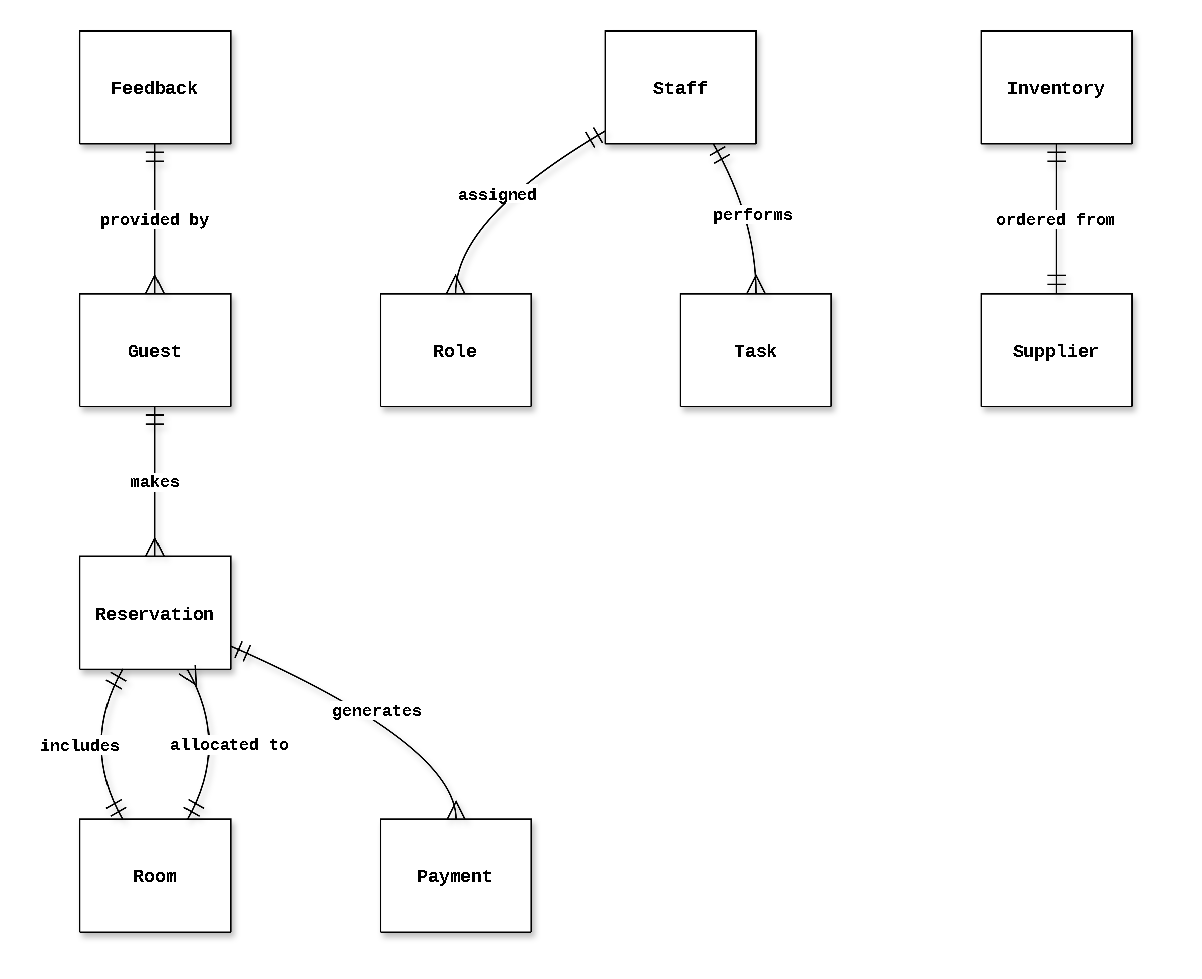
\includegraphics[width=\textwidth]{Conceptuat-ERD.pdf}
\caption{Conceptual ER Diagram}
\end{figure}

\begin{figure}[h]
\centering
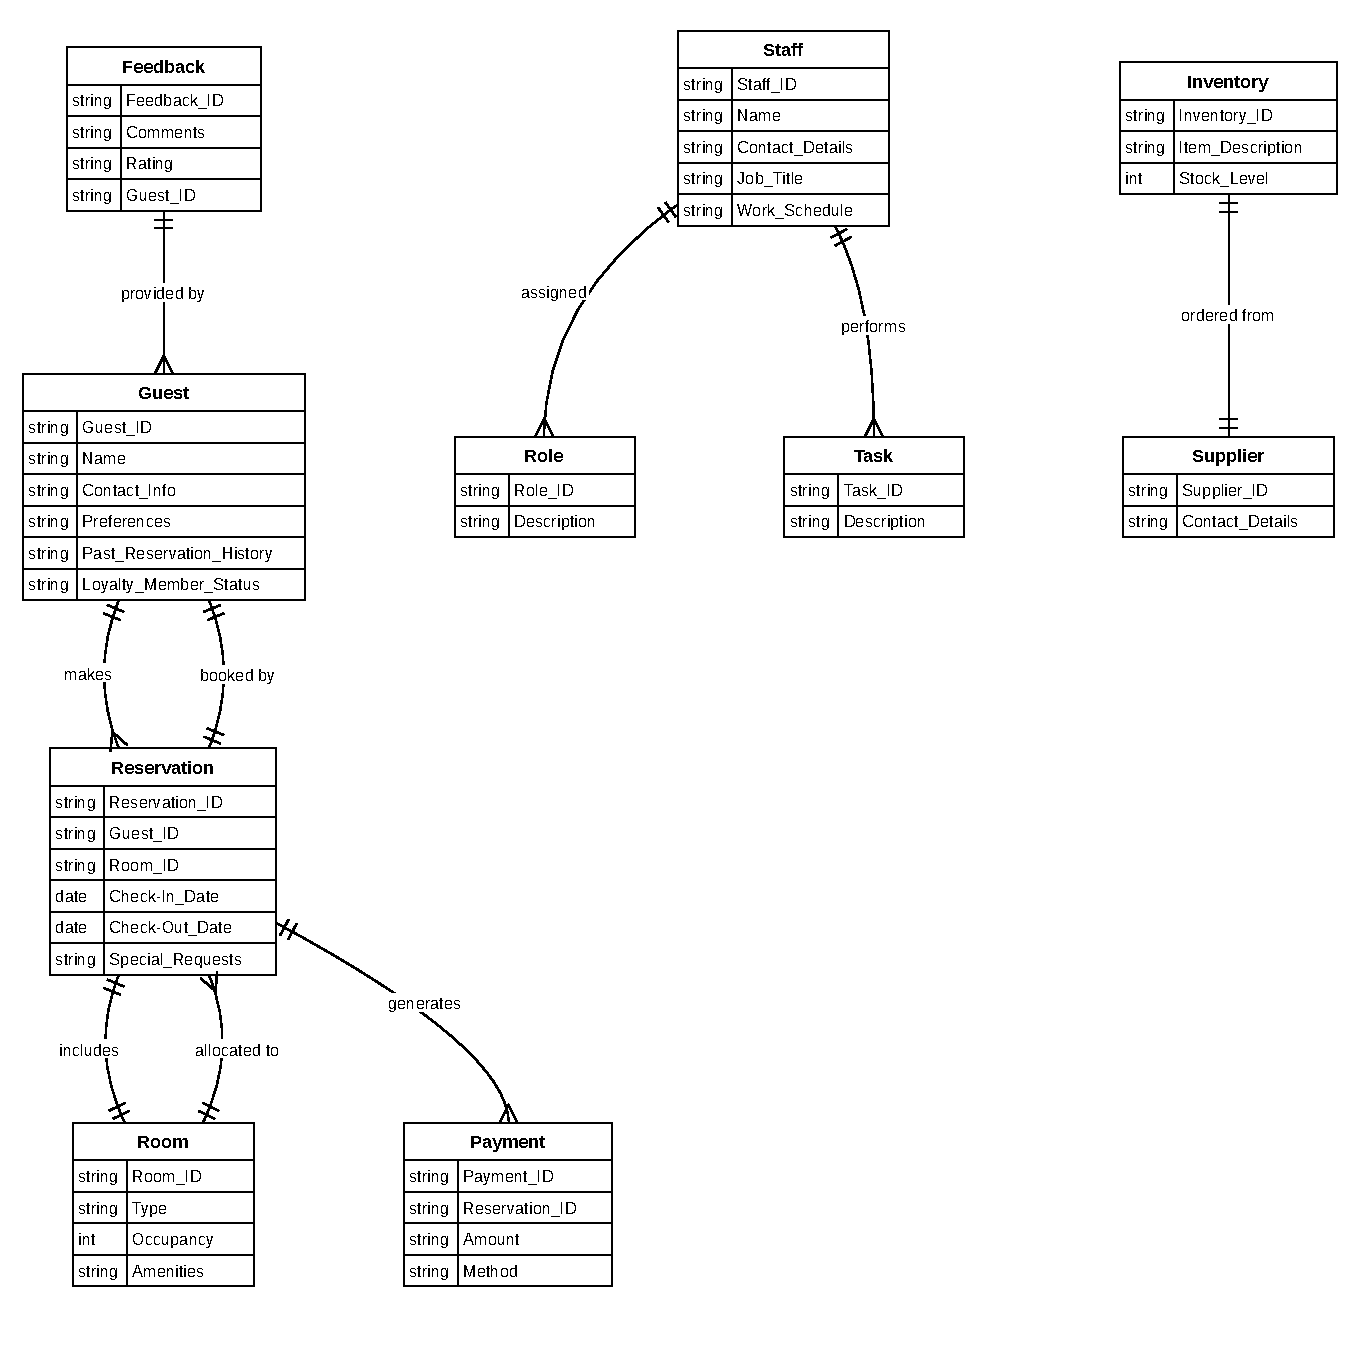
\includegraphics[width=\textwidth]{Logical-ERD.pdf}
\caption{Logical ER Diagram}
\end{figure}

\newpage


\begin{figure}[h]
\centering
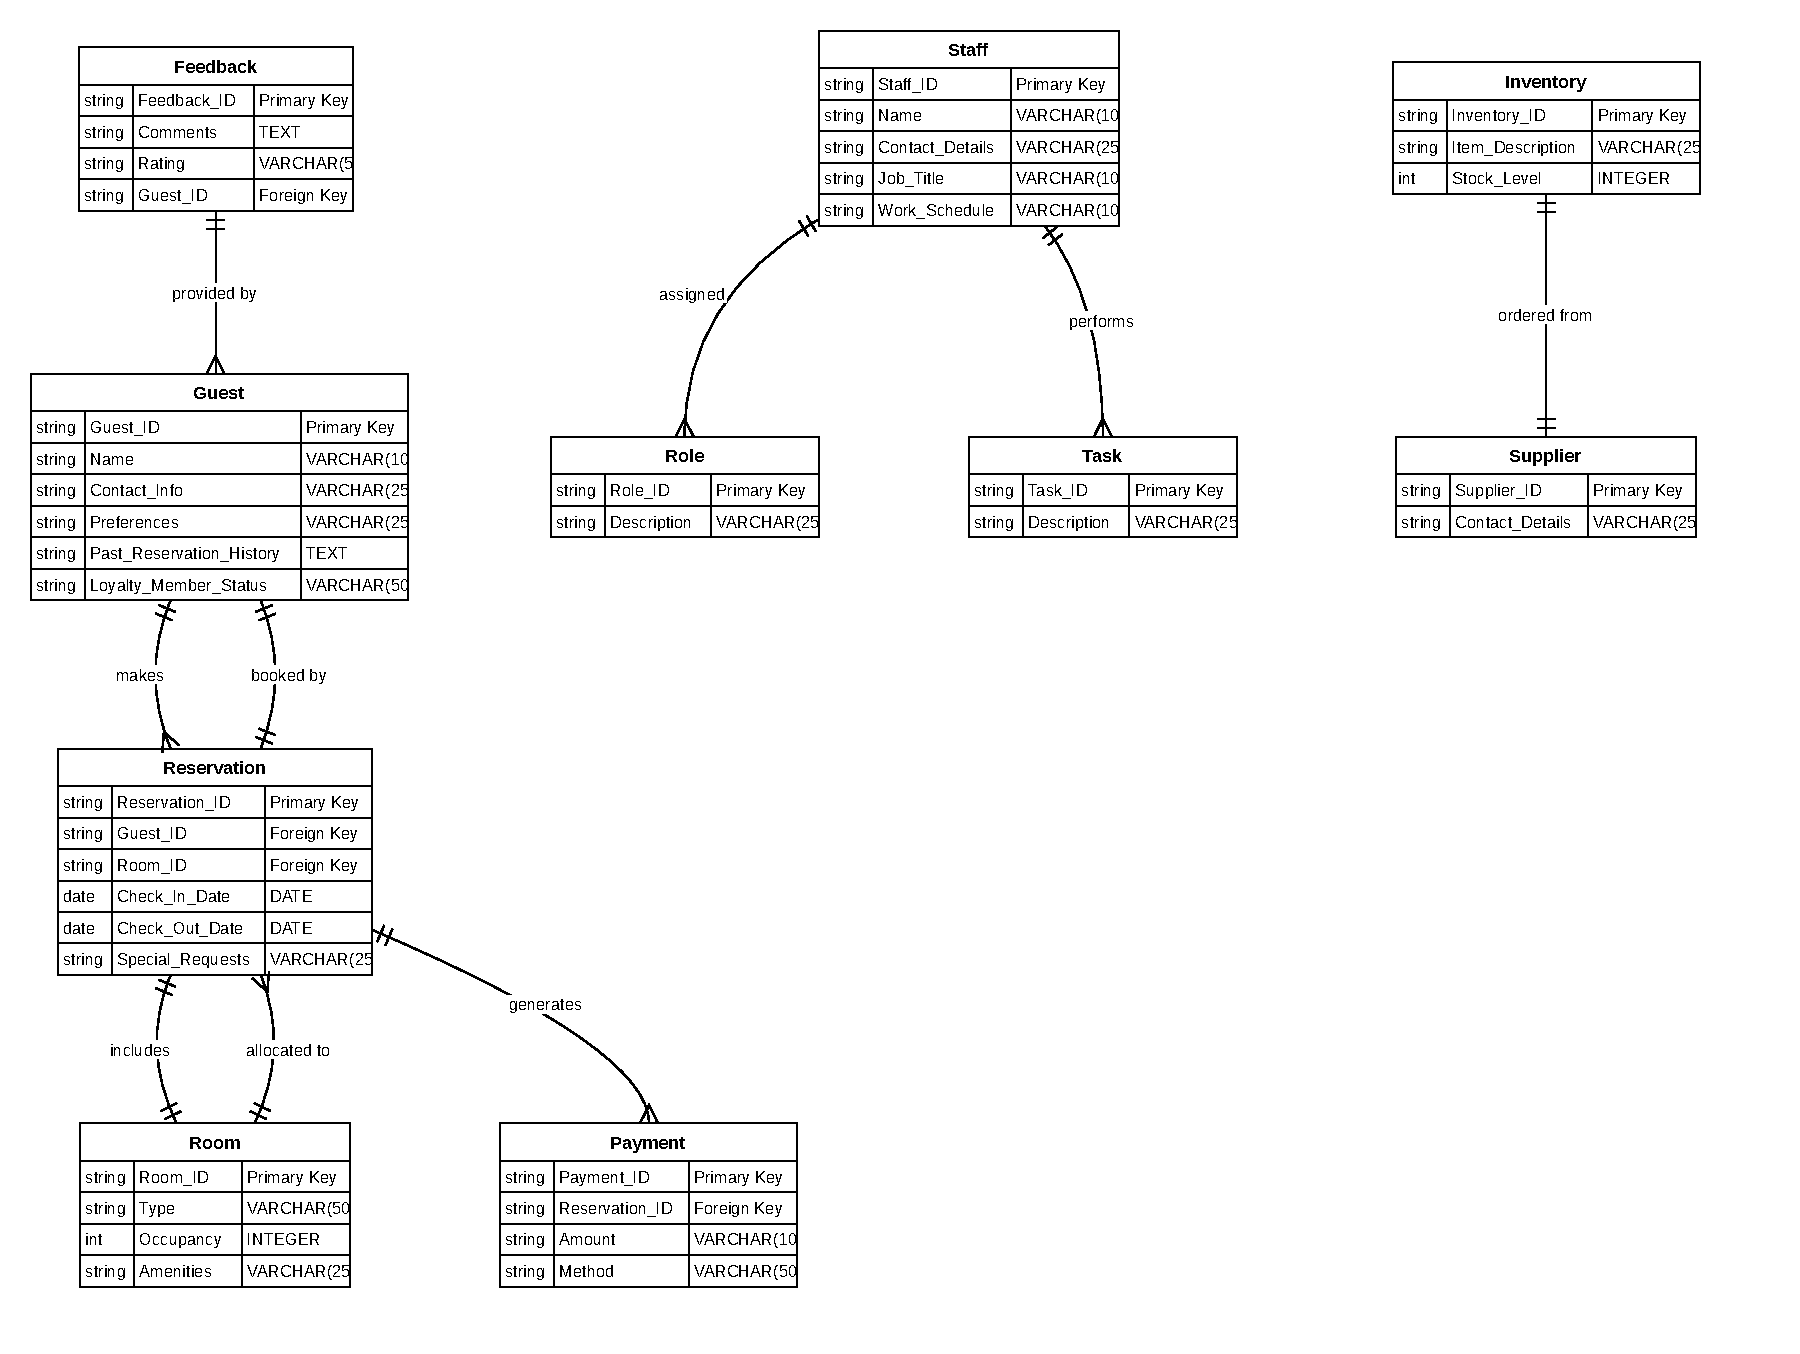
\includegraphics[width=\textwidth]{physical_erd.pdf}
\caption{Physical ER Diagram}
\end{figure}

\newpage


\section*{Tool Selection}
I chose Amazon RDS with AWS codecatalyst tool over MySQL Workbench for its online tool nature. It provides syntax support for all database languages and works with any notation of an ERD, making our development workflow easy, regardless of the tediousness of tool installation.
\end{document}
